% Integer and half-integer reflection mirrors for Z semidirect C2.
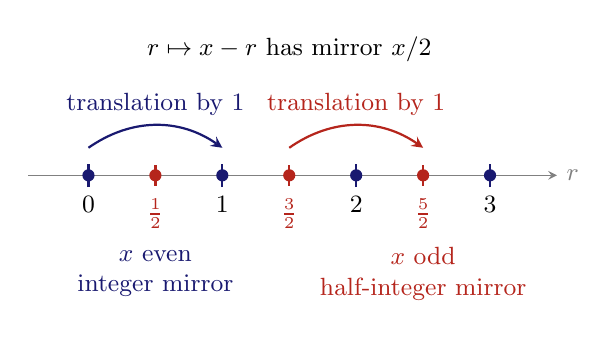
\begin{tikzpicture}[font=\small,>=stealth,x=1.7cm,y=1cm]
\draw[->,gray] (-0.45,0) -- (3.5,0) node[right] {$r$};
\foreach \x in {0,1,2,3} {
  \draw[MidnightBlue,thick] (\x,-0.15) -- (\x,0.15);
  \fill[MidnightBlue] (\x,0) circle (2.2pt);
  \node[below] at (\x,-0.15) {$\x$};
}
\foreach \x in {0.5,1.5,2.5} {
  \draw[BrickRed,thick] (\x,-0.13) -- (\x,0.13);
  \fill[BrickRed] (\x,0) circle (2.2pt);
}
\node[below,BrickRed] at (0.5,-0.18) {$\frac12$};
\node[below,BrickRed] at (1.5,-0.18) {$\frac32$};
\node[below,BrickRed] at (2.5,-0.18) {$\frac52$};
\draw[->,thick,MidnightBlue] (0,0.35) to[bend left=35] node[above] {translation by $1$} (1,0.35);
\draw[->,thick,BrickRed] (1.5,0.35) to[bend left=35] node[above] {translation by $1$} (2.5,0.35);
\node[MidnightBlue,align=center] at (0.5,-1.25) {$x$ even\\integer mirror};
\node[BrickRed,align=center] at (2.5,-1.25) {$x$ odd\\half-integer mirror};
\node[align=center] at (1.5,1.6) {$r\mapsto x-r$ has mirror $x/2$};
\end{tikzpicture}
